\documentclass[dvipdfmx]{beamer}


%%%%% VIEW %%%%%
\usetheme{Montpellier}
\usecolortheme{crane}
\usefonttheme{professionalfonts} % Math Font
\setbeamertemplate{footline}[frame number] % only frame number in footer
\setbeamertemplate{navigation symbols}{} % remove navigation symbol
\renewcommand{\familydefault}{\sfdefault}% font chenge to Sans-serif in English
\usepackage[deluxe,expert]{otf}
\renewcommand{\kanjifamilydefault}{mg}% font chenge to hiragino in Japanese

\setbeamertemplate{caption}[numbered]
%%%%% Fiture, Table Title Rename %%%%E%
\renewcommand{\figurename}{図}
\renewcommand{\tablename}{表}

\usepackage{bm} % Bold charactor package for math
\usepackage{color}

\usepackage[footnotesize, bf]{caption}
\newcommand{\argmin}{\mathop{\rm arg~min}\limits}

%%%% Definition %%%%%
\usepackage{amsmath,amssymb}
\usepackage{amsthm}
\theoremstyle{definition}

\title{PRML Seminar \#1}
\subtitle{ 1.1-1.6.1 \quad \#PRML学ぼう}
\author{Shunya Ueta}
\institute{Graduate School of SIE, Univ. of Tsukuba \\ Department of Computer Science}
\date{\today} % Print Build time

%%%%% Start Slide part %%%%%

\begin{document}

\begin{frame}
  \titlepage % Generated Title Page by preamble params
\end{frame}

\begin{frame}
  \tableofcontents % Generated tabele of contents by section tag
\end{frame}

\section{Introduction}

\begin{frame}
  \frametitle{自己紹介}
    \begin{itemize}
      \item 名前:上田隼也(@hurutoriya)
      \item 筑波大学大学院1年(予定) \\
      \item 情報数理研究室所属
      \item 研究分野 : 画像認識・機械学習
    \end{itemize}
\end{frame}

\subsection{この勉強会について}

\begin{frame}
  \frametitle{この勉強会について}
  \begin{itemize}
    \item パターン認識と機械学習についての輪講です \\
    機械学習とパターン認識の基礎を理解、実用レベルで使いこなせ事を目的にセミナーを開催していきます
    \item 2015年を目処に一周予定
    \item 受講者には基礎的な微積分・線形代数・確率統計の知識を前提としています
    \item 資料中のサンプルコードはPythonを採用しています。
    \item 勉強会に関する情報については Hashtag: \textcolor{blue}{\#PRML学ぼう} を使って発信していきます
  \end{itemize}
\end{frame}

\subsection{PRML Seminar \#1 内容}
\begin{frame}
  \frametitle{今回の内容}
  PRML輪講の予定と発表担当者の策定
  \begin{figure}[htb]
    \centering
    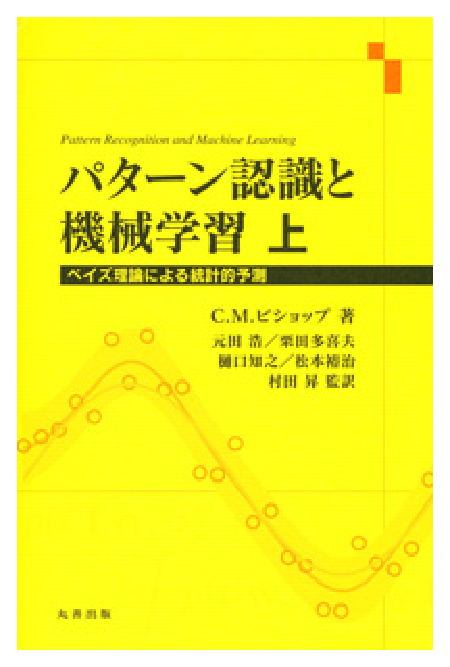
\includegraphics[width=2.5cm,clip]{res/prml.eps}
  \end{figure}
\end{frame}

\section{第$1$章 \enspace 序論}

\begin{frame}
  \frametitle{機械学習とは?}
  パターン認識(Pattern Recognition): \\ 計算機アルゴリズムを通じて、データの中の規則を\textcolor{blue}{自動的}に見つけ出す。更にその規則性を用いてデータを異なるカテゴリに分類する。
  \\
  例) 手書き数字の認識
   
  入力として$28 \times 28$ の大きさの手書き数字の画像がある。入力データは$784$次元の実数値ベクトル$x$で表現できる。ベクトル$\bm{x}$を入力として受け取り、それが$0 \ldots 9 $のどの数字を表しているかを出力する機械を作る。
  \begin{figure}[htb]
    \centering
    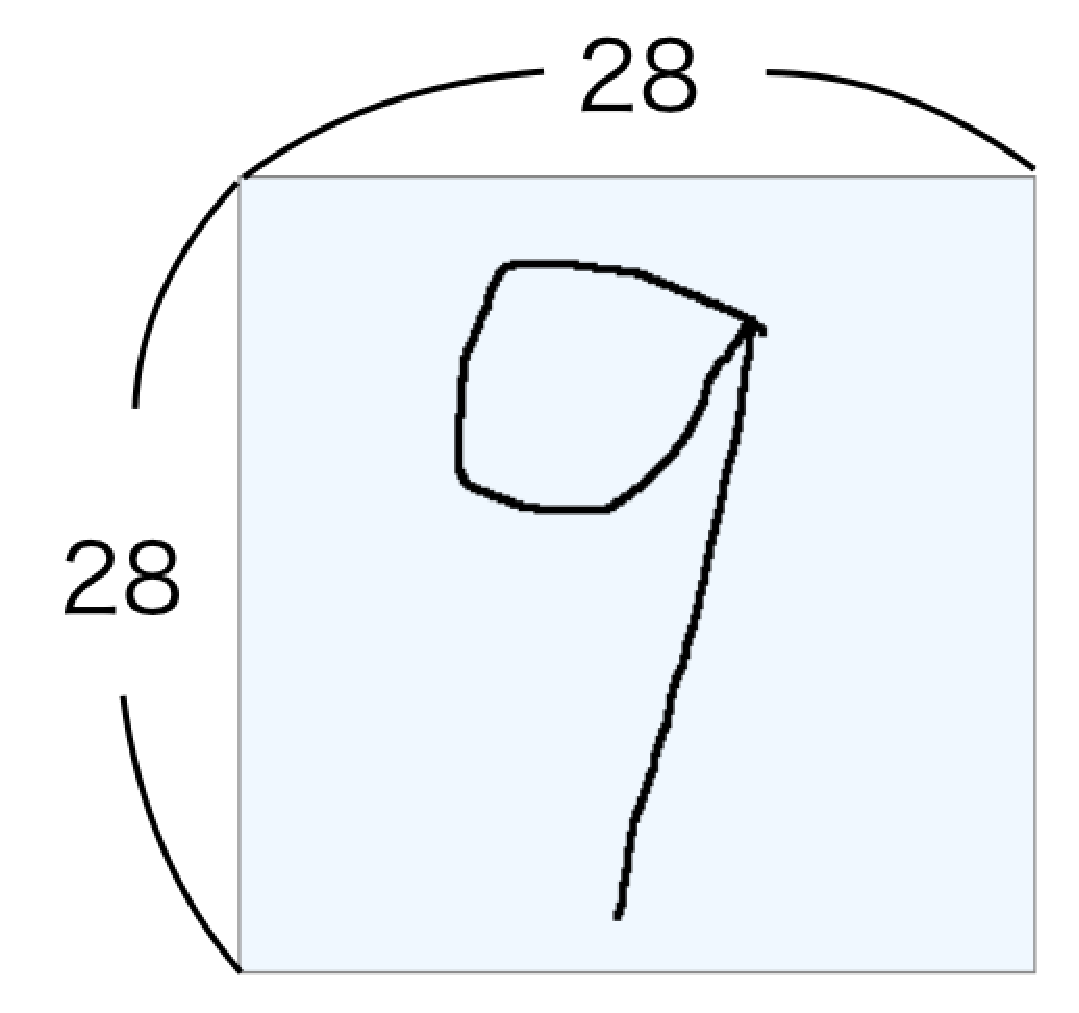
\includegraphics[width=1.5cm,clip]{res/handwritten.eps}
    \caption{手書き数字の画像例}
  \end{figure}
\end{frame}

\begin{frame}
  \frametitle{実現方法(1)}
  人力によるルールの作成 $\to$
  ルール数の発散(\textcolor{red}{実現不可})
  \\
  
  \begin{block}{機械学習的アプローチ}
    \begin{itemize}
      \item 訓練集合(training set):\\$N$個の手書き文字の大きな集合を用意する
      $\{x_1, \ldots , x_N \}$
      \item  目標ベクトル(target vector): $\bm{t}$ \\
      一つ一つの数字に対応するカテゴリを表すベクトル
    \end{itemize}
  \end{block}
  最終的に得られるのは$y(x)$である。\\
  この関数に数字の画像$\bm{x}$を入力すると、目標ベクトルと画像データに符号化可能なデータが合成されたベクトル$\bm{y}$(目標ベクトル)がラベリングされた画像が返ってくる。
\end{frame}

\begin{frame}
  \frametitle{実現方法(2)}
    \begin{itemize}
      \item 訓練(training), 学習(leaning) 段階 : \\ training setのみでモデル化されている状態
      \item テスト集合(test set) : \\ 訓練集合以外のデータ(未知のデータ)
      \item 汎化(generalization) : \\ 訓練集合以外のデータ(未知のデータ)に対して適応可能にさせること
    \end{itemize}
     実問題として入力データは大きな多様性を持つ。$\to$ \\ 汎化が中心的な課題となる。
\end{frame}

\begin{frame}
  \frametitle{例)Ajaxを使った手書き文字認識}
  \begin{figure}[htb]
    \centering
    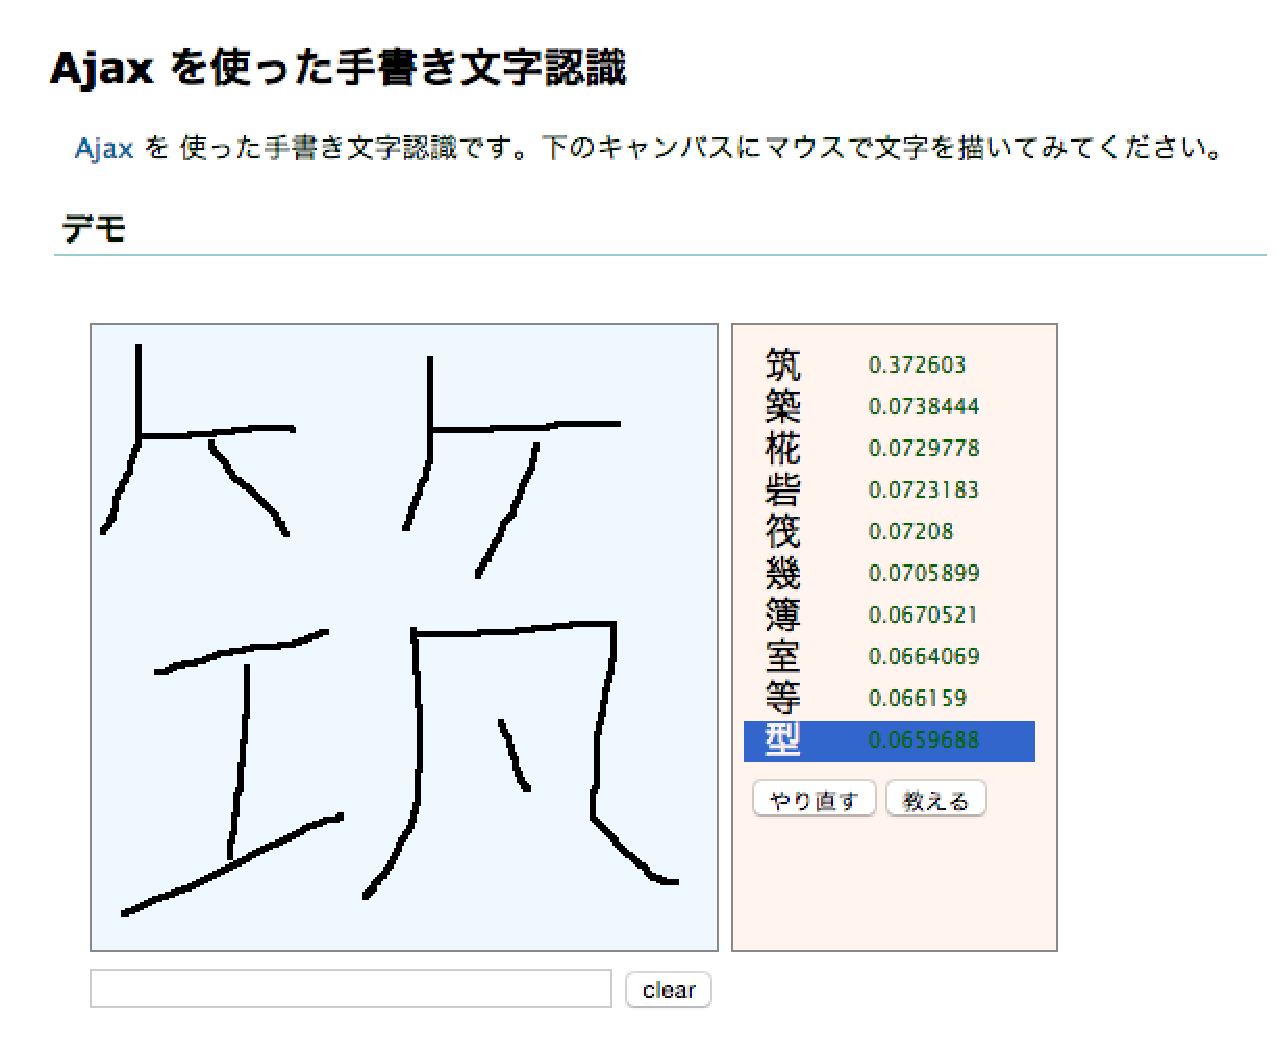
\includegraphics[width=6.0cm,clip]{res/ajax.eps}
    \caption{Ajaxを使った手書き文字認識}
  \end{figure}
  参考: \textcolor{blue}{http://chasen.org/~taku/software/ajax/hwr/}
\end{frame}

\begin{frame}
  \frametitle{前処理(Preprocessing)}
  実世界では、入力変数は\textcolor{blue}{前処理(Preprocessing)}により問題を解きやすくしておく。
  \begin{block}{例)手書き数字}
    \begin{itemize}
      \item 数字画像に変形(アフィン変換)、拡大・縮小を行い \\ 同一の大きさに変換 $\to$ 入力データの多様性の減少
    \end{itemize}
  \end{block}
  前処理の段階は特徴抽出(feature extraction)と呼ばれる。
  
  多様性減少の目的以外にも、計算の高速化のためにも用いられる事が多い。
\end{frame}

\begin{frame}
  \frametitle{機械学習の分類}
  \begin{enumerate}
    \item 教師あり学習(supervised learning) : 訓練データがラベリングされている状態での問題
      \begin{itemize}
        \item クラス分類(classification)問題 : 各入力ベクトルを有限個の離散カテゴリに分類する問題
        \item 回帰(regression) : 求める出力が一つないしはそれ以上の連続変数であるような問題
      \end{itemize}
    \item 教師なし学習(unsupervised learning) : 訓練データがラベリングされている状態での問題
      \begin{itemize}
        \item クラスタリング(clustering) : 類似した事例のグループを見つける
        \item 密度推定(density estimation) : 入力空間におけるデータの分布を見つける
      \end{itemize}
    \item 半教師あり学習(semis-upervised learning) : 訓練データがラベリングされているものと非ラベリング状態の物が混在している状態での問題
  \end{enumerate}
\end{frame}

\begin{frame}
  \frametitle{強化学習(reinforcement learning)(1)}
  教科学習(reinforcement learning) : ある与えられた条件下で、報酬を最大化するような適当な行動を見つける問題。
  \\
  状態と行動の系列から環境との相互作用を通じて学習を行う(行動基準は直近の報酬だけではなく、過去の行動も参考にされる)。
  \\
  教師あり学習との違い : 最適な答えは与えられずに試行錯誤を通じて学習アルゴリズム自らが最適解を発見する

  \begin{block}{バックギャモンに対する強化学習の適用(Tesauro 1994)}
    ニューラルネットワーク(第5章)により、自分自身のコピーと何百万ものゲームをこなす必要がある。\\
    選択肢は無数に存在するが、勝利という形でしか報酬を与えることができない。そのため、勝利に関係する手に対しては正確に報酬を割り当てる必要がある(\textcolor{red}{信頼度割り当て問題})。
  \end{block}
\end{frame}

\begin{frame}
  \frametitle{強化学習(reinforcement learning)(2)}
  下記の2つを行い強化学習を行う(トレードオフの関係)。
  \begin{itemize}
    \item 探査(exploration) : 新規の手がどれほど有効なのかを探す
    \item 利用(exploitation) : 高い報酬が得られることがわかっている行動を取る
  \end{itemize}
\end{frame}

\begin{frame}
  \frametitle{第1章で導入する3つの重要な道具}
  \begin{enumerate}
    \item 確率論
    \item 決定理論
    \item 情報理論
  \end{enumerate}
\end{frame}

\subsection{1.1 多項式曲線フィッティング}
\begin{frame}
  \frametitle{1.1 \ 多項式曲線フィッティング}
  訓練データ \\
  入力 : $N$個の観測値$x$を並べた $\bm{x} = (x_1, \dots, x_N)^T$ \\
  出力 : それぞれに対応する観測値 $\bm{t} = (t_1, \dots, t_N)^T$ \\
 
  未知の入力変数$x$に対して目標変数を予測したい$t$ (汎化)\\
  
  目標とするモデルは$\sin{2 \pi x}$、訓練データはノイズを乗せて$N=10$で与えられる。
  \begin{figure}[htb]
    \centering
    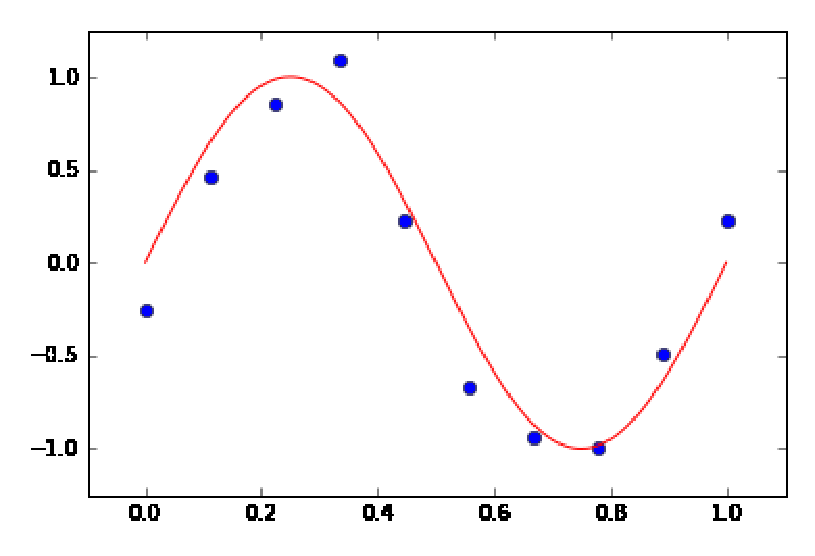
\includegraphics[width=4.0cm,clip]{res/fitting.eps}
    \caption{ex)N=10で訓練データが与えられている}
  \end{figure}
  
\end{frame}

\begin{frame}
  \frametitle{1.1 \ 多項式曲線フィッティング}
  \begin{gather*}
    y(x,\bm{w}) = w_0 x^0 + w_1 x^1 + \dots + w_M x^{M} = \sum_{j=0}^{M} w_j x^j
  \end{gather*}
  $M$:多項式の次数(order) \\
  $\omega$:多項式の係数、まとめて$\bm{\omega}$で表す \\
  \begin{gather*}
    E(\bm{w}) = \frac{1}{2} \sum_{n=1}^{N} \{ y(x_n,\bm{w})- t_n \}^2
  \end{gather*}
  訓練データに多項式をあてはめることで、係数の値を求めたい $\to$ 誤差関数(Error Function)の最小化を目指す。
\end{frame}

\begin{frame}
  \frametitle{Fitting Order Case:M=0,1}
\end{frame}

\begin{frame}
  \frametitle{Fitting Order Case:M=3,9}
\end{frame}

\begin{frame}
  \frametitle{過学習と平均二乗平方根誤差}
  9次でフィッティングした場合、\textcolor{red}{過学習}(over-fitting)
  \\
  \textcolor{blue}{機械学習の目標}:未知のデータに対して精度の高い予測(汎化)
  \begin{gather*}
    E_{RMS} = \sqrt{2E(\bm{w})/N}
  \end{gather*}
  平均二乗平方根誤差(root-mean-square error,RMS error)
  \\
  \begin{itemize}
    \item Nで割ることでサンプル数のギャップを消す
    \item 平方根を取ることで、元の尺度に戻す
  \end{itemize}
\end{frame}
\begin{frame}
  \frametitle{データセットのサイズに応じた過学習の様子}
\end{frame}
\begin{frame}
  \frametitle{誤差関数の正則化(regularization)過学習を制御}
  \begin{gather*}
    E(\bm{w}) = \frac{1}{2} \sum_{n=1}^{N} \{ y(x_n,\bm{\omega})- t_n \}^2 + \frac{\lambda}{2}||\bm{w} ||^2
  \end{gather*}
  2次の正則化の場合、リッジ回帰(ridge regression)
\end{frame}

\begin{frame}
  \frametitle{}
  検証用集合(Validation set):$\bm{w}$を決定するためにデータセット ホールド・アウト集合(hold-out set)とも呼ばれる。
  
  \textcolor{red}{欠点}: 貴重なデータを無駄にする
\end{frame}

\subsection{1.2 確率論}

\begin{frame}
  \frametitle{確率論}
  データにはノイズが必ず付随し、データセットのサイズも有限である。\textcolor{red}{不確実性}が重要な概念となる。
  
  \begin{block}{確率論の概念を簡単に説明}
    \begin{figure}[htb]
      \centering
      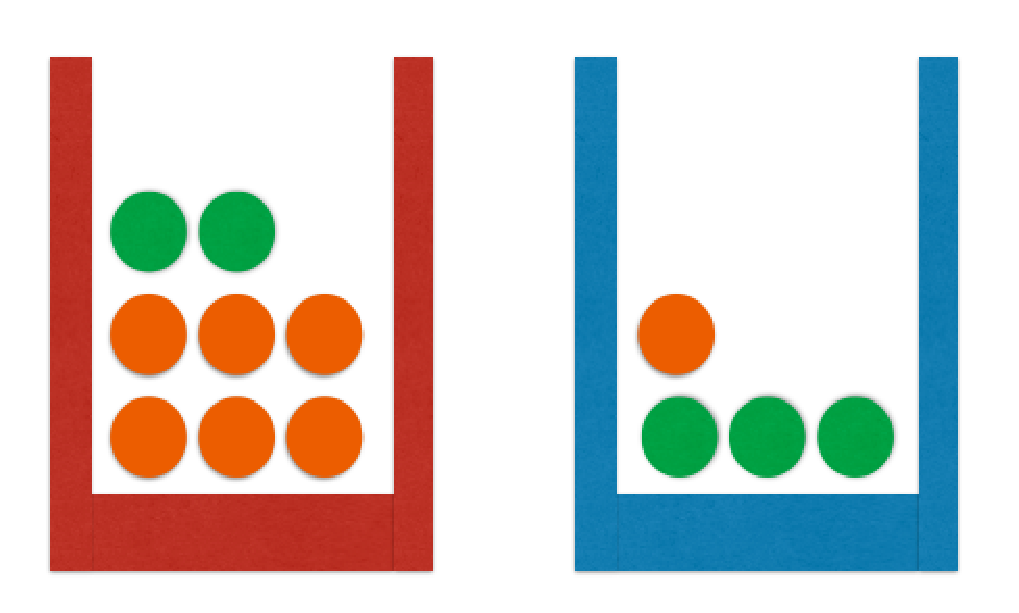
\includegraphics[width=4.0cm,clip]{res/probability.eps}
      \caption{赤と青、2つの箱がある。赤の箱にはりんごが2個、オレンジが6個、青の箱にはりんごが3個、オレンジが一個入っている。赤の箱を40\%,青の箱を60\%で選び、果物は同じ確からしさで選ぶ。}
    \end{figure}
  \end{block}
\end{frame}

\begin{frame}
  \frametitle{確率の基本的法則}
  \begin{itemize}
    \item 確率の加法定理
    \item 確率の乗法定理
  \end{itemize}
\end{frame}
\begin{frame}
  \frametitle{}
\end{frame}
\begin{frame}
  \frametitle{}
\end{frame}
\begin{frame}
  \frametitle{}
\end{frame}
\begin{frame}
  \frametitle{}
\end{frame}
\begin{frame}
  \frametitle{}
\end{frame}
\begin{frame}
  \frametitle{}
\end{frame}

\end{document}
